\textit{DAE simulation functionality in Matlab}

The simulation of the chemical reactions are presented as follows:

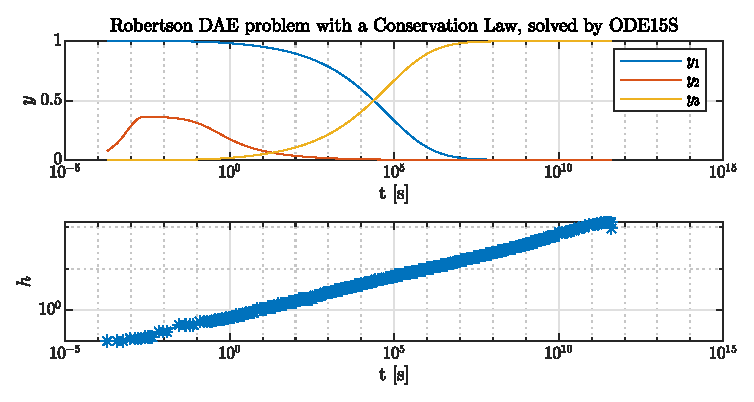
\includegraphics[width=\textwidth]{Figures/Ugf233.eps}

The code is given as follows:

\begin{lstlisting}
	clc; clear all;
	
	p1 = 0.04; p2 = 10e4; p3 = 3e7; % Constants 
	y0 = [1; 0; 0]; % initial conditions
	
	% function definition
	robertsdae = @(t,y) [-p1*y(1) + p2*y(2).*y(3); 
	p1*y(1) - p2*y(2).*y(3) - p3*y(2).^2;
	y(1) + y(2) + y(3) - 1 ];
	
	% simulation
	tsim = [0 40e10]; % simulation time
	M = [1 0 0; 0 1 0; 0 0 0]; % Mass matrix
	options = odeset('Mass',M);
	% play with the tols and try with ode15i
	
	[t,y] = ode15s(@(t,y) robertsdae(t,y),tsim,y0,options);
\end{lstlisting}

It is worth mentioning that the initial conditions are computed internally when we use the \texttt{ode15s} solver. However, another approach is to use the implicit solver \texttt{ode15i} and the initial conditions are given by using the function \texttt{decic}.